\chapter{软件设计实现}\label{chap:software}

硬件设计不是唯一的难点,本章节将详细概述 NVDLA 的软件栈的构建,首先我们需要为 ZYNQ 器件移植 Linux 操作系统,其次需要将 NVDLA 的驱动程序挂载到 Linux 内核中,然后需要编译出用户程序,最后,由于 NVDLA 的 small 配置仅支持 INT8 格式的数据,本章还将介绍结合 TensorRT 的模型量化方法。

\section{NVDLA 软件工具链概述}

如图~\ref{fig:NVDLA Software},NVDLA 的软件工具链分为 Compiler 和 Runtime 两个部分。

\begin{figure}[!htbp]
    \centering
    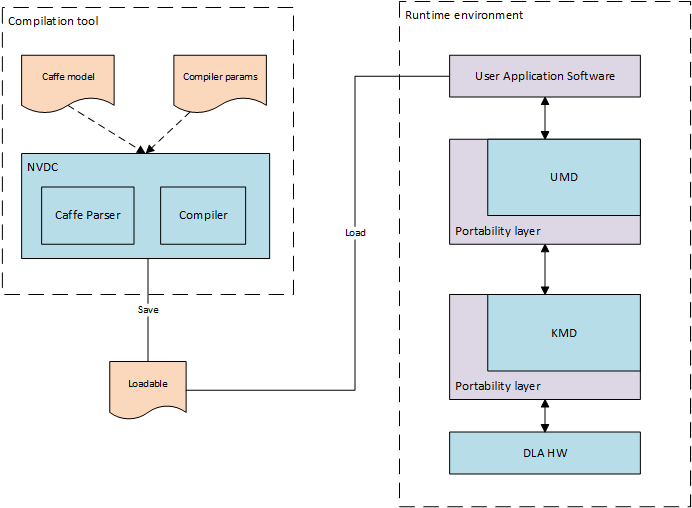
\includegraphics[width=0.7\textwidth]{software_package.png}
    \caption{NVDLA Software}
    \label{fig:NVDLA Software}
\end{figure}

Compiler 与硬件无关,可以在主机运行。它可以接受其他深度神经网络训练框架训练完成的模型,完成一些硬件无关的优化,例如算子融合、数据重用等,并且使用 FlatBuffers 将处理结果封装成 Loadable 数据流文件。

Runtime 与硬件紧密结合,其负责接受 Compiler 生成的 Loadable 文件,调度加速器程序,自动分配内存,自动配置寄存器,自动处理中断。而 Runtime 内部又被划分为两个部分,UMD 和 KMD吗,分别对应了 Linux 的用户态驱动与内核驱动。

\begin{itemize}
    \item 用户态驱动程序(USER MODE DRIVER,UMD)由 C++ 编写,负责解析 Loadable 文件,分配内存,并将上下文封装成一个 Task,最后发送给底层的 KMD 程序执行。
    \item 内核态驱动程序(KERNEL MODE DRIVER)由 C 语言编写,是 NVDLA 固件的驱动程序,他是真正与 NVDLA 进行交互的部分。
\end{itemize}

在这一小节,我们将详细的介绍 NVDLA 的软件工具链。如图~\ref{fig:NVDLA Software},英伟达官方提供了完整的软件生态。


Compiler 是软件工具链的前端,与硬件无关,Compiler 能够接受的参数如下:

\begin{lstlisting}
./nvdla_compiler -h
Usage: ./nvdla_compiler [-options] --prototxt <prototxt_file> --caffemodel <caffemodel_file>
where options include:
    -h                                                 print this help message
    -o <outputpath>                                    
    --profile <basic|default|performance|fast-math>    computation profile
    --cprecision <fp16|int8>                           compute precision
    --configtarget <nv_full|nv_large|nv_small>         target platform
    --calibtable <int8 calib file>                     
    --quantizationMode <per-kernel|per-filter>         
\end{lstlisting}

\begin{itemize}
    \item profile 指定了优化方案,在 Compiler 内部提供了四种优化方案,能够支持一些硬件无关的网络优化,例如算子融合、内存重用等,本设计使用默认的 fast-math,启用全部的优化选项。
    \item cprecision 指定了精度,在这里我们需要选择 int8,并且可以结合 TensorRT 生成 calibtabel 文件,如果不给出 calibtabel 参数,Compiler 内部会使用简单的量化方案,但在实际测试情况下,效果并不理想。
    \item configtarget 本设计选择 nv\_small,匹配本设计的 small 配置。
    \item calibtabel 需由 TensorRT 生成,将在下一小节详细介绍。
    \item quantizationMode 有两个选项,per-kernel 选项是对每一层卷积使用相同的量化参数,per-filter 则是对每一层卷积使用不同的量化参数,这需要结合 calibtabel 文件选择,在本设计中使用 per-kernel。
\end{itemize}

最终,Compiler 生成 Loadable 文件,交给 Runtime 进行加速器的调度。

Loadable 文件是 Compiler 与 Runtime 之间通信的媒介,其由 Google 开源的 FlatBuffers 序列化协议所组织,能够将对象与数据进行压缩,以便在网络中进行传输。简单来讲,我们需要在流中传输一个对象,比如网络流。一般我们需要把这个对象序列化之后才能在流中传输(例如,可以把对象直接转化为字符串),然后在接收端进行反序列化(例如把字符串解析成对象)。但是显然把对象转成字符串传输的方法效率十分低下,于是有了各种流的转换协议,FlatBuffers也是其中一种。

Runtime 与硬件紧密贴合,其又分为 UMD 和 KMD 两个部分:UMD 是用户应用,需要我们在 Linux 上编译运行,其接受 Loadable 文件并解析,最后递交一个推理任务到 KMD;KMD 是内核驱动,需要我们在构建 Linux 的时候编译,运行 Linux 的时候挂载,接受推理任务之后负责调度网络,配置寄存器,处理中断等任务。Runtime 能够接受的参数如下:

\begin{lstlisting}
./nvdla_runtime -h
Usage: ./nvdla_runtime [-options] --loadable <loadable_file>
where options include:
    -h                    print this help message
    -s                    launch test in server mode
    --image <file>        input jpg/pgm file
    --normalize <value>   normalize value for input image
    --mean <value>        comma separated mean value for input image
    --rawdump             dump raw dimg data
\end{lstlisting}

Compiler 的编译过程较简单,本设计不多介绍,Runtime 的构建过程非常复杂,将在后面的章节详细介绍。

\section{TensorRT 与模型量化}

本设计使用的 small 配置,仅支持 INT8 的推理,而 Caffe 框架仅支持 Float32 类型的训练,所以我们必须进行模型的量化。前文提到,在 Compiler 中量化需要结合英伟达公司的 TensorRT 框架。

\subsection{TensorRT 量化原理}

将高精度的浮点型转化为八比特的定点类型的量化方法,都遵循如下的公式:

$$ T_F = SF * T_I + B $$


其中$T_F$指 Float 类型的张量、$SF$指 Scale Factor、$B$指偏置 Bias,通过实验测得,Bias 去掉对精度的影响不大,最终该公式变为:

$$ T_F = SF * T_I $$

综合以上,进行神经网络的量化,本质上是求得每个参数的 Scale Factor 。最简单的量化方案是 max-max 映射:

$$ SF = \frac{|W|_{max}}{128} $$

将权重数据根据绝对值的最大值作为阈值,归一化到 -128 到 127之间,该方法针对分布均匀的权重数据是很有效果的。但是很明显,如果权重数据分布不均匀,该方法带来的精度损失很大。

TensorRT 选择的量化方法是 KL-divergence,即转化为最小化相对熵的问题\cite{shen2019highly}。相对熵表述的就是两个分布的差异程度,在量化问题上表述的是量化前后两个分布的差异程度,而我们的问题自然而然就代表着差异最小。关于求解的算法本设计不阐述,实际上英伟达也只是公开了解决方案,但是软件算法实现并没有开源,在 TensorRT 中我们也是只能调用其封装好的链接库。

\subsection{量化步骤与精度损失}

使用 TensorRT 进行量化的宏观处理流程如下,首先准备一个校准数据集,然后对每一层进行 Float32 的推理,之后依次:

\begin{enumerate}
    \item 收集激活值的直方图;
    \item 基于不同的阀址产生不同的量化分布;
    \item 然后计算每个分布与原分布的相对熵,然后选择熵最小的一个,也就是跟原分布最像的一个;
\end{enumerate}

校准是核心部分,校准数据集可以从训练集或者验证集中采样,本设计选择从验证集中进行采样方便对比精度损失情况,关于采样多少张图片,英伟达官方建议采样 500 到 1000 张图片。

本文设计并且量化了三个网络:

\begin{enumerate}
    \item 针对 MNIST 数据集的 Lenet5
    \item 针对 CIFAR10 数据集的 Resnet18
    \item 针对 IMAGENET2012 数据集的 Resnet18
\end{enumerate}

这些网络的结构与量化样例代码略复杂,在附录里给出了 Lenet5 网络的量化关键代码,除此之外仅给出量化前后的精度损失情况,如表~\ref{tab:Qualifications Report}。

\begin{table}[!htbp]
    \caption{TensorRT 量化精度损失}
    \label{tab:Qualifications Report}
    \centering
    \footnotesize% fontsize
    \setlength{\tabcolsep}{4pt}% column separation
    \renewcommand{\arraystretch}{1.2}%row space 
    \begin{tabular}{lcc}
        \toprule
        \textbf{Network}      & \multicolumn{1}{l}{\textbf{Valiadation Accuracy \%}} & \multicolumn{1}{l}{\textbf{Calibration Accuracy \%}} \\
        \midrule
        Lenet5-MNIST          & 99.7                                                 & 99.5                                                 \\
        Resnet18-CIFAR10      & 90.2                                                 & 86.7                                                 \\
        Resnet18-IMAGENET2012 & 60.2(Top5)                                           & 50.5(Top5)                                           \\
        \bottomrule                   
    \end{tabular}
\end{table}

\subsection{calibtabel 生成}

使用 TensorRT 量化会生成 cache 文件,内部每一行代表每一个 layer 的 Scale Factor ,但是 NVDLA 的 Compiler 在进行量化时需要接受 Json 格式的文件,其结构如下:

\begin{lstlisting}
    {"first_conv":
        {"scale": 1.0007381439208984,
         "max": 0,
         "offset": 0,
         "min": 0
        }
    },
\end{lstlisting}

其中 first\_conv 是 Layer 的 name,遗憾的是,英伟达官方没有提供正常可用的 Cache 到 Json 转换的脚本,本设计使用 Python3 结合 PyCaffe 自行编写了 Cache 文件到 Json 文件转化的脚本,该脚本的内容详见附录。

这样,我们就可以生成针对 small 配置的 Loadable 文件,只要将 Loadable 与输入 Image 准备好,就可以使用 Runtime 自动调度加速器进行推理,接下来介绍 Runtime 的上板编译过程。

\section{Ubuntu 16.04 根文件系统移植}

\subsection{Petalinux 工具介绍}

Xilinx Petalinux 是一个定制版的 Yocto 工具,包括了Linux Kernel、u-boot、device-tree、rootfs等源码、库,可以让客户很方便的生成、配置、编译及自定义。Petalinux支持Zynq UltraScale+ MPSoC、Zynq-7000全可编程SoC,以及MicroBlaze,可与Xilinx硬件设计工具Vivado协同工作,大大简化了Linux系统的开发工作。

使用PetaLinux工具,开发人员可以定制u-boot、Linux内核或Linux应用,开发者还可以通过网络或JTAG在随附的全系统仿真器 (QEMU) 或物理硬件上添加新的内核、器件驱动程序、应用和库,以及启动并测试软件协议栈,完成从系统启动到执行的所有操作。在主机端提供的PetaLinux工具包括:

\begin{itemize}
    \item 命令行界面
    \item 应用、器件驱动程序、库生成器以及开发模板
    \item 可引导的系统镜像生成器
    \item 调试代理程序
    \item GCC工具集
    \item 集成的QEMU全系统仿真器
    \item 自动化工具
    \item 支持Xilinx系统调试器
\end{itemize}

本设计将基于 Petalinux 2019.1 (Linux Kernel 版本为 4.19)完成 KMD 环境的移植与 UMD 应用的编译,由于 NVDLA 官方仓库的代码是针对 Linux Kernel 4.13 与 64位架构处理器的,其有一些函数已经在本内核函数中被废弃,还有一些操作在本设计采用的 32位 处理器上不被允许,这些问题都将在本章得到解决。

Petalinux 不具备包管理工具,为了更方便开发与调试,本章将介绍 Ubuntu 16.04 的根文件系统替换方法,为板卡移植 Ubuntu 操作系统,并且在这个过程中阐述 Petalinux 的构建方法。

\subsection{读取 Block Design 配置信息}

由于本设计需要将根文件系统替换为 Ubuntu 16.04,首先需要做的是将根文件系统与 Boot 文件分离,在 Petalinux 项目构建时,需要配置从 SD 卡中读取根文件系统。

使用 \emph{petalinux-config} 命令,指定上一章节生成的硬件描述文件的路径,在 \emph{Image Packaging Configuration|Root Filesystem Type},选中SD card,然后进行编译。

\begin{lstlisting}
petalinux-config --get-hw-description=./PathOfhdf
\end{lstlisting}

修改此处后,linux 根文件系统 rootfs 将配置到 SD 中,而非默认的  raminitfs,后者是将根目录系统镜像在 boot 阶段加载到内存中,一旦裁剪的kernel较大(大概超过120M),那么系统 boot 不起来。

\subsection{Linux 内核裁剪}

由于我们已经将 rootfs 配置到 SD 中,那么就要取消掉 kernel 的 RAM intial,否则在 boot 阶段,kernel 在内存中找不到 rootfs 的符号镜像。

\begin{lstlisting}
petalinux-config -c kernel
\end{lstlisting}

使用该命令配置取消 \emph{Initial RAM filesystem and RAM disk support} 。

\subsection{生成 Boot 和 Image 文件}

这样我们就可以进行编译,生成适配板卡的 BOOT 和 Image 文件,已经 rootfs 文件系统了,使用以下命令进行编译与生成,注意,这里我们还没有挂载 NVDLA 的硬件驱动,仅移植 Ubuntu 文件系统。

\begin{lstlisting}
petalinux-build
petalinux-package --boot --fsbl images/linux/zynq_fsbl.elf --fpga --u-boot --force
\end{lstlisting}

这样,BOOT.BIN 与 IMAGE.ub 文件以及 ROOTFS 将会在目录下生成。

\subsection{SD 卡分区}

本设计使用了一张 32 GB 大小的 SD 卡,因为前文配置了 rootfs 从 SD 卡启动,所以我们需要对 SD 卡进行分区,分区情况如表~\ref{tab:SD Card Partition}所示。

\begin{table}[!htbp]
    \caption{SD 卡分区}
    \label{tab:SD Card Partition}
    \centering
    \footnotesize% fontsize
    \setlength{\tabcolsep}{4pt}% column separation
    \renewcommand{\arraystretch}{1.2}%row space 
    \begin{tabular}{lccc}
        \toprule
        \textbf{Volume Name} & \multicolumn{1}{l}{\textbf{Type}} & \multicolumn{1}{l}{\textbf{Device}} & \multicolumn{1}{l}{\textbf{Space GB}} \\
        \midrule
        BOOT                 & FAT32                             & /dev/sdc1                                & 4                                \\
        ROOTFS               & EXT4                              & /dev/sdc2                                & 20                               \\
        WorkSpace            & EXT4                              & /dev/sdc3                                & 8                                \\
        \bottomrule                   
    \end{tabular}
\end{table}

其中,BOOT 分区格式为 FAT32,用来存储 BOOT.BIN 和 IMAGE.ub 文件,ROOTFS 需要的空间较大,用来存储根文件系统,WorkSpace 可有可无,我们使用他作为一个外置的存储,来存储一些数据。根据 Petalinux 的用户手册,BOOT 和 ROOTFS 需要严格在第一分区与第二分区。

\subsection{替换根文件系统}

本设计不采用 Petalinux 自己生成的根文件系统,使用 \emph{ubuntu-16.04.2-minimal-armhf-2017-06-18} 作为根文件系统,将其解压到 rootfs 分区,再将 BOOT.BIN 与 IMAGE.ub 文件拷贝到 BOOT 分区,将 SD 卡插入开发板则移植成功。

\section{KMD 内核程序挂载}

在上一小节,本文讲解了如何利用 Petalinux 为 ZYNQ 器件移植 Ubuntu 的操作系统,在这一小节,我们将为 Ubuntu 增加 NVDLA 的内核驱动程序。

\subsection{新增 Linux 设备树节点}

使用 Petalinux 构建操作系统的时候会自动为我们生成设备树文件,但是他只包括了一些基本的硬件属性。本设计考虑到 NVDLA 的内核驱动程序,对设备树文件做以下更改:

\begin{enumerate}
    \item 为 NVDLA 保留 256 MB 内存,因为在内核驱动程序中使用 DMA 搬移数据加快访存速度。
    \item 将原本 PL 侧的 NVDLA 的设备树的 compatible 属性修改以适应内核驱动程序。
\end{enumerate}

更改后的设备树文件详见附录 \emph{system-user.dtsi}。

\subsection{Petalinux 内核应用添加}

使用 Petalinux 内建的工具即可新增内核应用,本设计创建了一个名为 opendla 的子模块:

\begin{lstlisting}
petalinux-create -t modules -n opendla --enable
\end{lstlisting}

将 NVDLA 官方的 KMD 内核应用程序进行移植,首先需要对源代码做如下更改。

\begin{enumerate}
    \item 在\emph{nvdla\_gem.c}里面,将\emph{dma\_declare\_coherent\_memory}函数所分配的内存大小更改为设备树中为 NVDLA 保留的内存。
    \item \emph{DMA\_MEMORY\_MAP } 标志已经在 Linux kernel 4.19 版本中被废弃,删除即可。
    \item 在\emph{nvdla\_core\_callbacks.c}中,求解运算时间使用到了64位除法,这在32位处理器的内核程序上是不被允许的,需要做一些改动。
\end{enumerate}

对 KMD 的源代码改动完毕之后,还需要重新组织文件结构,使其适应 Petalinux 的模块构建方案,此外还需要重新编写 opendla 模块目录下的 \emph{Makefile} 与 \emph{opendla.bb} 文件,这两个文件的详细内容见附录。

修改完成后,重新进行编译,生成的内核驱动文件会在 Linux 根文件系统的 \emph{/lib/modules} 目录下,该文件会生成在 Petalinux 自己的根文件系统中,我们需要将其解压到 Ubuntu 的根文件系统的相同目录下。

\subsection{驱动程序加载}

启动系统之后,即可在 Ubuntu 中进行驱动程序的挂载:

\begin{lstlisting}
insmod /lib/modules/4.19.0-xilinx-v2019.1/extra/opendla.ko 
\end{lstlisting}

加载成功之后,可以看到系统设备中会多出 NVDLA 的中断信号和驱动。

\section{UMD 应用程序编译}

内核驱动挂载成功之后,我们的 UMD 程序才可以正确运行,而 UMD 也可分为两个主要部分:

\begin{itemize}
    \item 第一部分负责解析提前编译好的 Loadable 文件,将权重、输入图像等数据导入内存,并指定输出图像的地址。
    \item 第二部分负责把任务发送给 KMD 执行。
\end{itemize}

在本小节将介绍如何在开发板卡上进行 UMD 应用程序的编译。

\subsection{LIBJPEG 链接库编译}

NVDLA 的 Runtime 可以接受 jpeg 格式文件的图片,但是需要提前编译好 LIBJPEG 的链接库。

官方提供的64位处理器的 LIBJPEG 链接库无法在32位处理器上链接所以我们需要自行编译,本设计使用最新发行的 libjpeg9b,还需要更改 \emph{jconfig.h} 中的 \emph{JPEG\_LIB\_VERSION}的值为 90。

\subsection{UMD 构建}

将自行编译的 libjpeg.a 文件拷贝到项目中来,则可以进行 UMD 应用的编译,将 UMD 文件都拷贝到开发板卡的 Ubuntu 上,执行以下命令即可完成编译:

\begin{lstlisting}
cd ~/umd
export TOP=${PWD}
make runtime TOOLCHAIN_PREFIX=/usr/bin/
\end{lstlisting}

完成编译后,会生成两个目录文件,分别为 runtime 的链接库与 runtime 的可执行文件。将 runtime 的链接库拷贝到 runtime 可执行文件路径下,runtime可执行文件才能被正常运行。

\subsection{Runtime 测试}

一切准备完毕之后,可以使用 resnet-18 推理一副小猫的照片进行测试:

\begin{lstlisting}
./nvdla_runtime --loadable ~/resnet18-cifar10-caffe/loadables/fast-math.nvdla --image ~/resnet18-cifar10-caffe/Image/cat_32.jpg --rawdump
creating new runtime context...
Emulator starting
dlaimg height: 32 x 32 x 3: LS: 256 SS: 0 Size: 8192
submitting tasks...
Work Found!
Work Done
execution time = 295854.000000 us
Shutdown signal received, exiting
Test pass
cat output.dimg 
0 0 0 99 26 0 0 0 0 0 
\end{lstlisting}

类别猫在 CIFAR10 数据集中的序号是3,分类正确,耗时 300 毫秒,这代表着软件栈能够正常工作。